% $Id: template.tex 11 2007-04-03 22:25:53Z jpeltier $

\documentclass{vgtc}                          % final (conference style)
%\documentclass[review]{vgtc}                 % review
%\documentclass[widereview]{vgtc}             % wide-spaced review
%\documentclass[preprint]{vgtc}               % preprint
%\documentclass[electronic]{vgtc}             % electronic version

%% Uncomment one of the lines above depending on where your paper is
%% in the conference process. ``review'' and ``widereview'' are for review
%% submission, ``preprint'' is for pre-publication, and the final version
%% doesn't use a specific qualifier. Further, ``electronic'' includes
%% hyperreferences for more convenient online viewing.

%% Please use one of the ``review'' options in combination with the
%% assigned online id (see below) ONLY if your paper uses a double blind
%% review process. Some conferences, like IEEE Vis and InfoVis, have NOT
%% in the past.

%% Figures should be in CMYK or Grey scale format, otherwise, colour 
%% shifting may occur during the printing process.

%% These few lines make a distinction between latex and pdflatex calls and they
%% bring in essential packages for graphics and font handling.
%% Note that due to the \DeclareGraphicsExtensions{} call it is no longer necessary
%% to provide the the path and extension of a graphics file:
%% 
\includegraphics{diamondrule} is completely sufficient.
%%
\ifpdf%                                % if we use pdflatex
  \pdfoutput=1\relax                   % create PDFs from pdfLaTeX
  \pdfcompresslevel=9                  % PDF Compression
  \pdfoptionpdfminorversion=7          % create PDF 1.7
  \ExecuteOptions{pdftex}
  \usepackage{graphicx}                % allow us to embed graphics files
  \DeclareGraphicsExtensions{.pdf,.png,.jpg,.jpeg} % for pdflatex we expect .pdf, .png, or .jpg files
\else%                                 % else we use pure latex
  \ExecuteOptions{dvips}
  \usepackage{graphicx}                % allow us to embed graphics files
  \DeclareGraphicsExtensions{.eps}     % for pure latex we expect eps files
\fi%

%% it is recomended to use ``\autoref{sec:bla}'' instead of ``Fig.~\ref{sec:bla}''
\graphicspath{{figures/}{pictures/}{images/}{./}} % where to search for the images

\usepackage{microtype}                 % use micro-typography (slightly more compact, better to read)
\PassOptionsToPackage{warn}{textcomp}  % to address font issues with \textrightarrow
\usepackage{textcomp}                  % use better special symbols
\usepackage{mathptmx}                  % use matching math font
\usepackage{times}                     % we use Times as the main font
\renewcommand*\ttdefault{txtt}         % a nicer typewriter font
\usepackage{cite}                      % needed to automatically sort the references
\usepackage{tabu}                      % only used for the table example
\usepackage{booktabs}                  % only used for the table example
%% We encourage the use of mathptmx for consistent usage of times font
%% throughout the proceedings. However, if you encounter conflicts
%% with other math-related packages, you may want to disable it.


%% If you are submitting a paper to a conference for review with a double
%% blind reviewing process, please replace the value ``0'' below with your
%% OnlineID. Otherwise, you may safely leave it at ``0''.
\onlineid{0}

%% declare the category of your paper, only shown in review mode
\vgtccategory{Research}

%% allow for this line if you want the electronic option to work properly
\vgtcinsertpkg

%% In preprint mode you may define your own headline.
%\preprinttext{To appear in an IEEE VGTC sponsored conference.}

%% Paper title.

\title{Towards interactivity with DViz}

%% This is how authors are specified in the conference style

%% Author and Affiliation (single author).
%%\author{Roy G. Biv\thanks{e-mail: roy.g.biv@aol.com}}
%%\affiliation{\scriptsize Allied Widgets Research}

%% Author and Affiliation (multiple authors with single affiliations).
%%\author{Roy G. Biv\thanks{e-mail: roy.g.biv@aol.com} %
%%\and Ed Grimley\thanks{e-mail:ed.grimley@aol.com} %
%%\and Martha Stewart\thanks{e-mail:martha.stewart@marthastewart.com}}
%%\affiliation{\scriptsize Martha Stewart Enterprises \\ Microsoft Research}

%% Author and Affiliation (multiple authors with multiple affiliations)
\author{Jodi Spacek\thanks{e-mail: jodi.spacek@gmail.com}\\ %
        \scriptsize University of British Columbia %
\and Stewart Grant\thanks{e-mail:sgrant09@cs.ubc.ca}\\ %
     \scriptsize University of British Columbia }

%% A teaser figure can be included as follows, but is not recommended since
%% the space is now taken up by a full width abstract.
%\teaser{
%  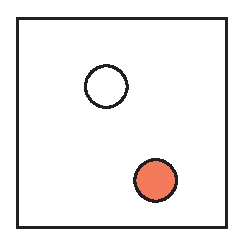
\includegraphics[width=1.5in]{sample.eps}
%  \caption{Lookit! Lookit!}
%}


\usepackage{ifthen}
\usepackage[normalem]{ulem} % for \sout
\usepackage{xcolor}
\usepackage{amssymb}

\newcommand{\ra}{$\rightarrow$}
\newboolean{showedits}
\setboolean{showedits}{true} % toggle to show or hide edits
\ifthenelse{\boolean{showedits}}
{
	\newcommand{\ugh}[1]{\textcolor{red}{\uwave{#1}}} % please rephrase
	\newcommand{\ins}[1]{\textcolor{blue}{\uline{#1}}} % please insert
	\newcommand{\del}[1]{\textcolor{red}{\sout{#1}}} % please delete
	\newcommand{\chg}[2]{\textcolor{red}{\sout{#1}}{\ra}\textcolor{blue}{\uline{#2}}} % please change
}{
	\newcommand{\ugh}[1]{#1} % please rephrase
	\newcommand{\ins}[1]{#1} % please insert
	\newcommand{\del}[1]{} % please delete
	\newcommand{\chg}[2]{#2}
}

\newboolean{showcomments}
%\setboolean{showcomments}{true}
\setboolean{showcomments}{false}
\newcommand{\id}[1]{$-$Id: scgPaper.tex 32478 2010-04-29 09:11:32Z oscar $-$}
\newcommand{\yellowbox}[1]{\fcolorbox{gray}{yellow}{\bfseries\sffamily\scriptsize#1}}
\newcommand{\triangles}[1]{{\sf\small$\blacktriangleright$\textit{#1}$\blacktriangleleft$}}
\ifthenelse{\boolean{showcomments}}
%{\newcommand{\nb}[2]{{\yellowbox{#1}\triangles{#2}}}
{\newcommand{\nbc}[3]{
 {\colorbox{#3}{\bfseries\sffamily\scriptsize\textcolor{white}{#1}}}
 {\textcolor{#3}{\sf\small$\blacktriangleright$\textit{#2}$\blacktriangleleft$}}}
 \newcommand{\version}{\emph{\scriptsize\id}}}
{\newcommand{\nbc}[3]{}
 \renewcommand{\ugh}[1]{#1} % please rephrase
 \renewcommand{\ins}[1]{#1} % please insert
 \renewcommand{\del}[1]{} % please delete
 \renewcommand{\chg}[2]{#2} % please change
 \newcommand{\version}{}}
\newcommand{\nb}[2]{\nbc{#1}{#2}{orange}}

\definecolor{ibcolor}{rgb}{0.4,0.6,0.2}
\newcommand\iv[1]{\nbc{IB}{#1}{ibcolor}}
\usepackage{wasysym}
\newcommand\yesml[1]{\nbc{ML {\textcolor{yellow}\sun}}{#1}{mircolor}}

\definecolor{sgcolor}{rgb}{0.2,0.0,0.5}
\newcommand\sg[1]{\nbc{SG}{#1}{sgcolor}}

\definecolor{samcolor}{rgb}{0.2,0.4,0.2}
\newcommand\sam[1]{\nbc{SC}{#1}{samcolor}}

\definecolor{hccolor}{rgb}{0.21,0.54,0.84}
\newcommand\hc[1]{\nbc{HC}{#1}{hccolor}}

% Todo Command
\definecolor{todocolor}{rgb}{0.9,0.1,0.1}
\newcommand{\todo}[1]{\nbc{TODO}{#1}{todocolor}}


%%%%%%%%%%%%%%%%%%%%%%%%%%%%%%%%%%%%%%%%%%%%%
\label{sec:abstract}
%%%%%%%%%%%%%%%%%%%%%%%%%%%%%%%%%%%%%%%%%%%%%
%% Abstract section.

\abstract{Understanding and debugging distributed systems is a
difficult task. Without proper tools developers are forced to inspect
logs from diverse machines. Tracing tools are used track distributed
executions based on control flow, and are typically accompanied by a
visualization front end for ease of use, and comprehension. Here we
propose a visualization for state based tracing. Our prior work used
t-SNE to visually cluster an execution. This approach took minutes on
traces of over 100 trace points, and over 300 variables, a significant
barrier to interactivity. In addition we used inferred data invariants
as a characterization of a systems properties. Lists of such
invariants totalled in the hundreds, and were incomprehensible to
users. Here we propose algorithmic, and architectural techniques for
improving the performance of t-SNE for the sake of interactivity, and
a novel technique for automatically extracting interesting data
invariants to reduce their cardinally, and increase
comprehensibility.}
%% end of abstract



%% ACM Computing Classification System (CCS). 
%% See <http://www.acm.org/class/1998/> for details.
%% The ``\CCScat'' command takes four arguments.

\CCScatlist{ 
  \CCScat{K.6.1}{Distributed Systems}%
{Trace Visualization}{Debugging Visualization};
}

%% Copyright space is enabled by default as required by guidelines.
%% It is disabled by the 'review' option or via the following command:
% \nocopyrightspace

%%%%%%%%%%%%%%%%%%%%%%%%%%%%%%%%%%%%%%%%%%%%%%%%%%%%%%%%%%%%%%%%
%%%%%%%%%%%%%%%%%%%%%% START OF THE PAPER %%%%%%%%%%%%%%%%%%%%%%
%%%%%%%%%%%%%%%%%%%%%%%%%%%%%%%%%%%%%%%%%%%%%%%%%%%%%%%%%%%%%%%%%
\begin{document}
\maketitle 
%%%%%%%%%%%%%%%%%%%%%%%%%%%%%%%%%%%%%%%%%%%%%
\section{Introduction and Motivation}
\label{sec:intro}
%%%%%%%%%%%%%%%%%%%%%%%%%%%%%%%%%%%%%%%%%%%%%


The complexities of distributed systems have long plagued their
developers. Writing code which executes on various machines is
intrinsically more complicated due to networking eccentricities, such
as failures, partitions, and message delays. Debugging and checking
the correctness of such systems is laborious and technical, as
developers must inspect large logs for small discrepancies in expected
values, and timestamps. At scale auxiliary tools are necessary for
interpreting logs and making them understandable. Typically tracing tools
are used to reconstruct the communication of nodes throughout a
system, order their events, and present developers with a
comprehensive view of an execution.
%%
    Tracing tools alone still produce large amounts of data, albeit
    their structure is more understandable than raw logs. Typically
    tracing tools are equipped with a visual front end, allowing users
    to quickly observe the behaviour of executions, and under scrutiny
    identify irregular or bugging behaviour. No one tracing technique
    is sufficient for debugging distributed systems. While most tracing
    tools are concerned with debugging they typically fall into 3 sub
    categories of performance tuning, distributed control flow, and
    model checking. Each of these tracing objectives have different
    flavors of visualization which pair with them. We overview these
    visualization techniques in Section~\ref{sec:related}
%%

We propose a tracing tool which captures state similar to a model
checking trace tools, with the exception that rather than logging
control flow, our tracing tool only logs a distributed programs state.
Such tracing is unconventional and does not fit nicely into the
aforementioned tracing categories. As such our unique requirements
demand innovative visualization solutions. Entirely state based program
analysis has ties in the world of trajectory
programming~\cite{Waterland:2014:AAS:2654822.2541985,181250,Waterland:2013:CC:2485732.2485749}.
In trajectory analysis simple ML techniques such as weather man, and
mean prediction, as well as linear, and logistic regression are used
to automatically predict and parrallelize computation based solely on
state analysis.

Our proposed visualization for traces of program state applies a
similar ML technique, t-SNE clustering, a dimensionality reduction
algorithm~\cite{Hinton_visualizingdata}. We leverage t-SNE to clusters
points in a programs execution based on the similarities of a programs
state.  T-SNE requires a distancing function to cluster state, our
distance function is as follows. The distance between two trace points
$p$ and $p'$, whose state is composed of an identical set of variables
with potentially different values. For each matching pair of variables
XOR them together. Each 1 bit in the resultant XOR is a difference of
1 bit between the variables. We calculate the difference between two
variables as the number of one bits in the XOR. The distance between
trace points $p$ and $p'$ is the euclidean norm of all variable
distances.

We found the results of our initial technique promising, and the high level
behaviour of distributed programs we traced. However, our visualization suffers
due to a high level of computational complexity in running t-SNE. A single step
of the iterative t-SNE algorithm is $O(n)$, and the algorithm is typically
executed for greater that 20 iterations before a reasonable clustering is
obtained. Typical runtimes for traces consisting of 80 - 100 trace points,
containing 80 - 100 variables each resulted in runtimes in the tens of minutes.
This significant barrier to interactivity lead us to alter the architecture of
our tool, and implement parallel t-SNE to achieve interactive sub 10s
computation times. 

Our prototype visualization allowed users to inspect trace points, and
view individual variable values, without the ability to compare
points. All variables were weighted equally when computing weights.
Our interactivity goals are two fold first developers should be able
to query two points, and inspect variables which caused them to be
distant from one another. Second we acknowledge that all variables are
not of equal importance in a program. Some variables values
drastically alter the behaviour of a program while other do not. To
this end we extended our interface to support re-clustering with
increased weights for important user specified variables.

An additional feature of our tracing tool is the analysis of
distributed data invariants. We infer invariants using Dinv, a
distributed front end for Daikon~\cite{Ernst99dynamicallydiscovering}.
These invariants are inferred over entire traces of an execution, and
the number of invariants can be large and incomprehensible (300-400).
In addition to our improvements of t-SNE we refined our invariant
analysis by first, logically detecting t-SNE clusters using k-Means
clustering, deriving per cluster invariants, and refining those
further to unique invariants for each cluster. This processing step
greatly reduces spurious, and uninteresting invariants, and profiles
cluster behaviour more precisely.

The rest of the paper is laid out as follows.
Section~\ref{sec:related} covers related work. Section~\ref{sec:scope}
overviews the scope of our contributions, and Section~\ref{sec:imp}
covers our implementation. Section~\ref{sec:res} details our
performance results and data refinement accuracy. Finally
Section~\ref{sec:dafw} and Section~\ref{sec:conclusion} denote
potential future work, and the conclusion of the paper.

%%%%%%%%%%%%%%%%%%%%%%%%%%%%%%%%%%%%%%%%%%%%%
\section{Scope}
\label{sec:scope}
%%%%%%%%%%%%%%%%%%%%%%%%%%%%%%%%%%%%%%%%%%%%%

Our initial distributed trace time curve visualization suffered a number of
shortcommings. Mainly the time to compute the time curve using tsne was too
slow, on the order of 8-10 minutes for the traces we wished to analyze. Such a
compute time is problematic for us because we wished to achive interactive
recomputation of the time curve by biasing clusters towards variables that
users marked as important. The leading cause of our visualizations compute time
was the single threaded JavaScript archetecture we used to run tsne. Another
shortcomming of our visualization was the lack of labels on clusters, and the
size of invariants generated for a single trace. T-SNE generates visual
clusterings, but not logicial ones, so no further computation can be done to
the clusters. Daikon, our tool for inferring distributed invariants, outputs
all of its template invariants which are not violated during an execution. This
number can be large, and many invariants are spurious. In the following section
we discribe our archetectural shift from JavaScript to Go, the implementation
of an effienct parrallel t-SNE, our back end support for skewing t-SNE
clustering towards important variables. Further, we disribe our algorithm for
computing visual t-SNE cluster into logical ones, our approach for calculating
cluster invariants, and their subset of unique cluster invariants.

\subsection{JavaScript to Go}
\label{sec:js2go}

JavaScript has many convienient frameworks for builing client server
applications which are compatable with nearly all browsers. This fact lead us
to develop our time curve prototype in a mixture of React~\cite{react}, and
node.js~\cite{node.js}. Calculating XOR distance on our target traces was
sufficiently slow with this framework that we cached results and served
precomputed distance from our node.js server. Figure\todo{reference orignal
javascript arcetecture} outlines our original archetecture. T-SNE coordinates
were calculated client side, at latencies of ~30s. To achieve our goal of
interactivity we desinged a new archetecture with a thin client, which issues
computation requests to an optimized server written in Go. Our choice of Go was
due to its concurrancy language primitives and increased performance. In
section ~\ref{sec:imp} we discuss the details of our implementation.

\subsection{Parallel t-SNE}
\label{sec:ptsne}
t-SNE is a ML algorithm for dimensionality reduction. We leverage t-SNE as the
state space of a trace point can be modeled as a high dimensional vector where
each variable is a dimension with a magnitude equal to it's binary encoding. At
it's core each itteration of t-SNE has 4 steps. First a cost gradent is
calculated, using a distance function, second the gradent is normalized, third
the gradent moves all projected points a distance, last the momentum of each
point is updated for the next step, and the points are reprojected. Each stage
of this algorithm has a data dependency on its prior step, therefore there is
no trivial method for parallizing t-SNE. Our solution requires that seperate
threads are delegated points for which they must compute values, and a master
thread which coordinates barriers to protected against inconsistant memory
accesses.



\noindent\textbf{XOR Distance:} A single point in a distributed trace can
consist of hundreds of variables.  Computing the distance between any
two points requires that we calculate XOR on each variable pair, and
then calculate the euclidean norm of each. Our typical traces consist
of ~100-300 variables per trace, and 100 trace points. As t-SNE is
$O(n^2)$ per itteration, requiring aproximatly 20 itterations for
reasonable results we end up with a typical number of XOR computations
in the order of ((300*300)/2)*100 * 20 ~100M XOR computations. We
aliviate much of this complexity by precomputing XOR distance for each
pairs of points and caching them. By doing so we only incur the full
cost of running XOR distance for a single itteration of t-SNE.


\subsection{variable weighting and distance reporting}

Figure~\ref{}\todo{make a graph with two unknown poitns} is an example
visualization generated by our original tool. At a glance the image is
composed of \todo{x} clusters, with no semantic meaning behind them.
In fact this is a distributed key value store responding to a 50\%
put, and 50\% get workload. Under the assumption that users would
generate their own traces from test cases, we assume that they will
have some understanding of the high level functional behaviour of
their system. To help developers reason precisely about clusters we
aimed to answer the question \emph{Why is point A distant from point
B?}.\todo{talk a bit about implementation?} 

\subsection{Cluster Detection, and Invariants}

The results of running t-SNE on high dimensional data are visual
clusters of points. While these points are usefull for descerning
patterns in a trace, but as they are visual, they are not available
for further analysis without an additional processing. We propose the
use of k-means clustering on t-SNE output, to logically cluster visual
clusters. Alternative density clustering techniques such as
DBSCAN~\cite{}\todo{cite dbscan} have greater precision at detecting
clusters automatically, our choice of k-means is to allow users to
select the number of clusters they observere.

\textbf{Cluster Invariants, and Unique Cluster Invariants}

Logical clusters detected by k-means, can be further prosessed in
isolation from other clusters. Our prototype tool output distributed
data invariants which held over an entire execution. These invariants
are course grain, and do not expose invariant behaviour of individual
clusters.  
%
Daikon outputs all template invariants which are not violated by a
trace, and which are supported by entries in a trace up to a minimal
confidence measure. Applying daikon to individual clusters has the
downside that the number of detected invariants grows, as there is
less evidence to invalidate spurious invariants. We propose that
invariants unique to clusters identify their most interesting
behaviour. To detect unique invariants we compair each cluster with
all others using Daikons \emph{Invariant Checker} tool. Unique
invariants for a cluster, are invariants which are violated by all
other clusters.




%%%%%%%%%%%%%%%%%%%%%%%%%%%%%%%%%%%%%%%%%%%%%
\section{Implementation}
\label{sec:imp}
%%%%%%%%%%%%%%%%%%%%%%%%%%%%%%%%%%%%%%%%%%%%%

%%%%%%%%%%%%%%%%%%%%%%%%%%%%%%%%%%%%%%%%%%%%%
\section{Results}
\label{sec:imp}
%%%%%%%%%%%%%%%%%%%%%%%%%%%%%%%%%%%%%%%%%%%%%


%%%%%%%%%%%%%%%%%%%%%%%%%%%%%%%%%%%%%%%%%%%%%
\section{Discussion and Future Work}
\label{sec:dafw}
%%%%%%%%%%%%%%%%%%%%%%%%%%%%%%%%%%%%%%%%%%%%%

\noindent\textbf{limitations}
            Our approach to visualizing distributed state is limited
            by computational power. Execution times of t-SNE grow
            polynomial with the length of a trace, therefore traces
            with lengths of tens of thousands would execute slowly
            regardless of parallelism. One heavy handed approach to
            gain scalability would be to spread out t-SNE computation
            on a cluster. However, the size of the trace would have to
            be in the tens of thousands to overcome the cost of
            synchronizing state.

            Logged state has a limited view of a programs behaviour.
            All state collected with our tracing technique must be at
            the application layer and not hidden within binaries. The
            more state which is logged, the better our clustering
            technique responds. Therefore, we are limited to
            applications where the majority of functionality, and
            interesting behaviour is resident in users application
            code. One potential solution to this problem would be to
            analyze a programs stack and heap at the OS layer. While
            this would provide a more holistic view of a programs
            state during execution it sacrifices important information
            such as variable names, log lines, not to mention a state
            space explosion.

            Allowing users to weight variables manually introduces the
            possibility of bias and error into our state model. Users
            with little experience of the programs they trace may be
            biased towards variables which are inconsequential, and
            could lead to their misunderstanding of a programs
            execution. This restricts our users to those which have a
            comprehensive knowledge of their software, and are in
            search of anomalies and bugs.

\noindent\textbf{future work}
            Clusters generated by t-SNE form a de facto state machine
            when connected temporally. Future work could extend our
            visualization to abstract clusters away, and present a
            state machine, where transitions between clusters were
            labeled with variables which caused them. The state of
            individual clusters could be simply encoded with their
            unique invariants.
        %
            Our current visualization is limited to a single
            execution. This approach may be useful for traces known
            to contain bugs, and abnormalities, but is arguably poor
            for checking subtle differences between multiple
            executions. Future work could cluster 2 or more executions
            together and compare their clustering transitions for
            similarities and differences. 

%%%%%%%%%%%%%%%%%%%%%%%%%%%%%%%%%%%%%%%%%%%%%
\section{Conclusion}
\label{sec:conclusion}

Here we presented a our work parallelizing t-SNE for the sake of
interactive clustering, and a proposed architecture for JavaScript
applications requiring fast responses, and large scale computation. We
improved the interactivity of our clustering visualization by allowing
users to re weight variables based on importance, and by justifying
point distances by reporting per variable distances.  addition we
presented our technique for reducing large scale invariant data in our
traces by applying k-means to t-SNE output, and logically analyzing the
unique invariant behaviour of clusters.

%%%%%%%%%%%%%%%%%%%%%%%%%%%%%%%%%%%%%%%%%%%%%


%% The ``\maketitle'' command must be the first command after the
%% ``\begin{document}'' command. It prepares and prints the title block.

%% the only exception to this rule is the \firstsection command

%% \section{Introduction} %for journal use above \firstsection{..} instead
This template is for papers of VGTC-sponsored conferences which are \emph{\textbf{not}} published in a special issue of TVCG.


%% if specified like this the section will be committed in review mode
\acknowledgments{
The authors wish to thank A, B, C. This work was supported in part by
a grant from XYZ.}

%\bibliographystyle{abbrv}
\bibliographystyle{abbrv-doi}
%\bibliographystyle{abbrv-doi-narrow}
%\bibliographystyle{abbrv-doi-hyperref}
%\bibliographystyle{abbrv-doi-hyperref-narrow}

\bibliography{template}
\end{document}
